%%%%%%%%%%%%%%%%%%%%%%%%%%%%%%%%%%%%%%%%%
% Beamer Presentation
% LaTeX Template
% Version 1.0 (10/11/12)
%
% This template has been downloaded from:
% http://www.LaTeXTemplates.com
%
% License:
% CC BY-NC-SA 3.0 (http://creativecommons.org/licenses/by-nc-sa/3.0/)
%
%%%%%%%%%%%%%%%%%%%%%%%%%%%%%%%%%%%%%%%%%

%----------------------------------------------------------------------------------------
%	PACKAGES AND THEMES
%----------------------------------------------------------------------------------------

\documentclass{beamer}

\mode<presentation> {
	
	% The Beamer class comes with a number of default slide themes
	% which change the colors and layouts of slides. Below this is a list
	% of all the themes, uncomment each in turn to see what they look like.
	
	%\usetheme{default}
	%\usetheme{AnnArbor}
	%\usetheme{Antibes}
	%\usetheme{Bergen}
	%\usetheme{Berkeley}
	%\usetheme{Berlin}
	%\usetheme{Boadilla}
	%\usetheme{CambridgeUS}
	%\usetheme{Copenhagen}
	%\usetheme{Darmstadt}
	%\usetheme{Dresden}
	%\usetheme{Frankfurt}
	%\usetheme{Goettingen}
	%\usetheme{Hannover}
	%\usetheme{Ilmenau}
	%\usetheme{JuanLesPins}
	%\usetheme{Luebeck}
	\usetheme{Madrid}
	%\usetheme{Malmoe}
	%\usetheme{Marburg}
	%\usetheme{Montpellier}
	%\usetheme{PaloAlto}
	%\usetheme{Pittsburgh}
	%\usetheme{Rochester}
	%\usetheme{Singapore}
	%\usetheme{Szeged}
	%\usetheme{Warsaw}
	
	% As well as themes, the Beamer class has a number of color themes
	% for any slide theme. Uncomment each of these in turn to see how it
	% changes the colors of your current slide theme.
	
	%\usecolortheme{albatross}
	%\usecolortheme{beaver}
	%\usecolortheme{beetle}
	%\usecolortheme{crane}
	\usecolortheme{dolphin}
	%\usecolortheme{dove}
	%\usecolortheme{fly}
	%\usecolortheme{lily}
	%\usecolortheme{orchid}
	%\usecolortheme{rose}
	%\usecolortheme{seagull}
	%\usecolortheme{seahorse}
	%\usecolortheme{whale}
	%\usecolortheme{wolverine}
	
	%\setbeamertemplate{footline} % To remove the footer line in all slides uncomment this line
	%\setbeamertemplate{footline}[page number] % To replace the footer line in all slides with a simple slide count uncomment this line
	
	%\setbeamertemplate{navigation symbols}{} % To remove the navigation symbols from the bottom of all slides uncomment this line
}

\usepackage{graphicx} % Allows including images
\usepackage{booktabs} % Allows the use of \toprule, \midrule and \bottomrule in tables

%----------------------------------------------------------------------------------------
%	TITLE PAGE
%----------------------------------------------------------------------------------------

\title[RP2040 Debugging]{Debugging an Embedded System} % The short title appears at the bottom of every slide, the full title is only on the title page
\subtitle{(The case for RP2040 and Picoprobe)}

\author{AITI} % Your name
\institute[AITI] % Your institution as it will appear on the bottom of every slide, may be shorthand to save space
{
	AITI \\ % Your institution for the title page
	\medskip
	\textit{renen@aiti-kace.com.gh} % Your email address
}
\date{\today} % Date, can be changed to a custom date

\begin{document}
	
	\begin{frame}
		\titlepage % Print the title page as the first slide
	\end{frame}
	
	\begin{frame}
		\frametitle{Overview} % Table of contents slide, comment this block out to remove it
		\tableofcontents % Throughout your presentation, if you choose to use \section{} and \subsection{} commands, these will automatically be printed on this slide as an overview of your presentation
	\end{frame}
	
	%\section{Objectives} 
	% Sections can be created in order to organize your presentation into discrete blocks, all sections and subsections are automatically printed in the table of contents as an overview of the talk
	%------------------------------------------------
	
	%----------------------------------------------------------------------------------------
	%	PRESENTATION SLIDES
	%----------------------------------------------------------------------------------------

	
	%------------------------------------------------

\section{Introduction}
\begin{frame}
	\frametitle{Introduction}
	\begin{block}{What is an Embedded System?}
		An embedded system is a computerized system that is purpose-built for its application. \\
		--\textbf{ Elecia White, Making Embedded Systems}
	\end{block}
	
	\begin{block}{What is an Embedded System?}
		A combination of computer hardware and software, and perhaps additional mechanical or other parts,
designed to perform a dedicated function. \newline
		-- \textbf{V. Gadre, Netaji University of Technology,New Delhi}
	\end{block}
\begin{block}{An embedded system}
	A computing system found in another system whose primary purpose is not computing.
\end{block}

\end{frame}

%------------------------------------------------
	
\begin{frame}
		\frametitle{Application areas}
		\begin{block}{Application areas}
			\begin{itemize}
				\item Robotics
				\item Telecommunication
				\item Sports
				\item Medicine
				\item Safety critical systems
			\end{itemize}
		\end{block}
	\begin{flushleft}
		\begin{figure}
			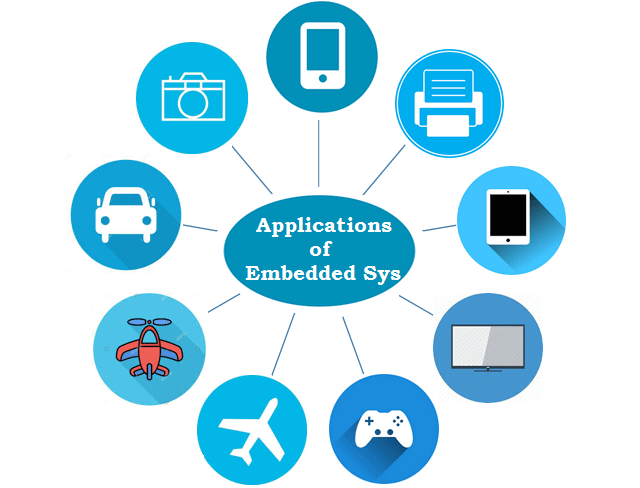
\includegraphics[width=0.5\linewidth,height=0.3\linewidth]{images/application.png}
		\end{figure}
	\end{flushleft}
\end{frame}

\begin{frame}{Debugging}
	\begin{block}{Debugging}
		The procedures through which engineers find and fix bugs(incorrect behaviour) in software(systems).
	\end{block}
\end{frame}


	\begin{frame}{From Code to Binary}

		\begin{block}{Embedded toolchain}
			In a compiler toolchain for a language like C/C++, there is :
			\begin{itemize}
				\item \textbf{Compiler}: Takes  source code in files and generates corresponding assembly code in files.
				\item \textbf{Assembler}: Takes assembly and produces machine code with no absolute addresses. 
				\item \textbf{Linker}: Takes machine code and links them against libraries and references from all files included in the project to produce a single binary file.
			\end{itemize}
		\end{block}
		Most times, invoking the compiler will call the subsequent steps in order.
	\end{frame}
	
	\begin{frame}{Embedded Programming Concepts}
		\begin{block}{Cross-compiling}
			Compiling code for an architecture different from the host CPU's architecture.\\
			Example: arm-none-eabi-gcc
		\end{block}
	\begin{figure}
		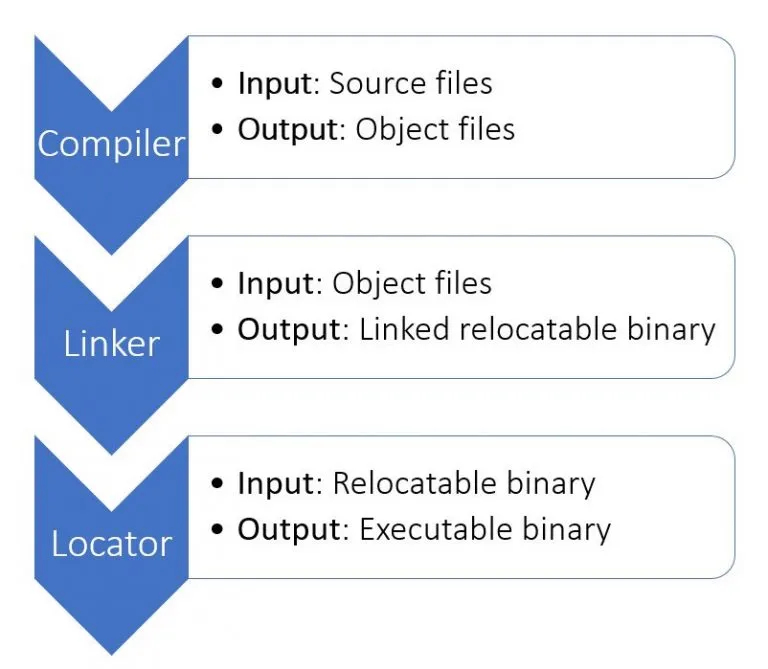
\includegraphics[width=.7\linewidth,height=.3\linewidth]{images/compilation_steps.jpg}
	\end{figure}

	\begin{block}{"Flashing"}
		Copying the resulting machine code in the right format(\textbf{.hex, .bin, .elf}) into non-volatile memory of the MCU.
	\end{block}
	\end{frame}

\section{Approaches to Debugging}
\begin{frame}{Approaches to Debugging}
		\begin{block}{Approaches}
		\begin{itemize}
			\item Logging over a serial port(printf debugging)
			\item Using a debugger
			\item Using a Logic Analyzer
			\item Oscilloscope, multimeter
		\end{itemize}
	\end{block}
\end{frame}

\section{Why use Hardware Debuggers?}
\begin{frame}{Why use Hardware Debuggers?}
	\begin{itemize}
		\item Ability to set breakpoints
		\item Step into, step out, step over, continue execution
		\item Inspect memory content (see values in variables during execution)
		\item Watch expressions
		\item printf debugging changes the timing(WS2812B might not work)
	\end{itemize}
\end{frame}


\begin{frame}{Hardware Debuggers}
	\begin{figure}
		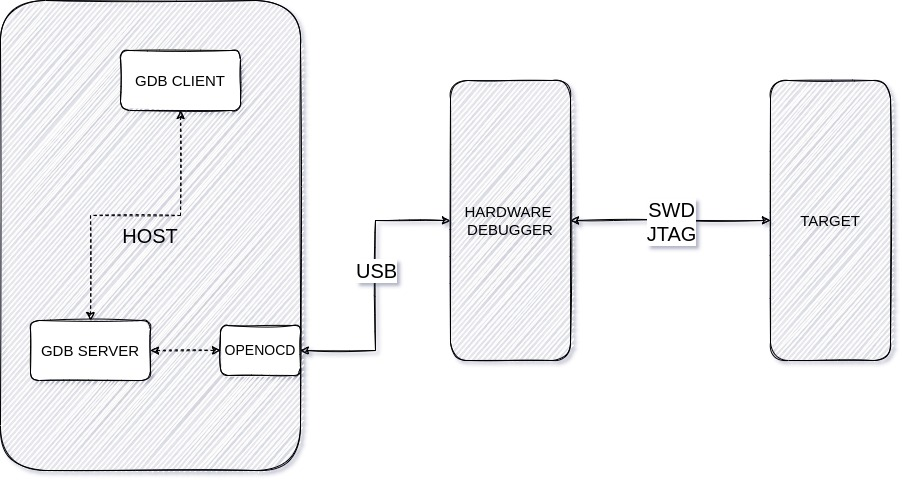
\includegraphics[width=.7\linewidth,height=.5\linewidth]{images/debugging.jpg}
	\end{figure}
\end{frame}
	
\begin{frame}{Hardware Debuggers -- Examples}
	\begin{block}{Examples}
		\begin{itemize}
			\item JLink Edu Mini(\$42.32)
			\item ST Link(\$20.00)
			\item Raspberry Pi(openocd) 
			\item Raspberry Pi Pico(picoprobe)(\$4.23)
		\end{itemize}
	\end{block}
\end{frame}

\begin{frame}{RP2040 }
	\begin{figure}
		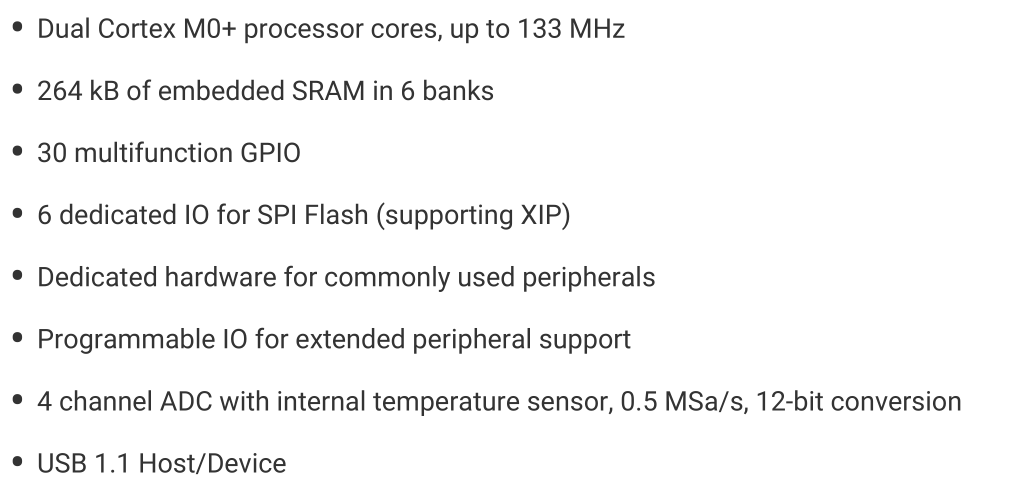
\includegraphics[width=.7\linewidth,height=.4\linewidth]{images/rp2040_specs.png}
	\end{figure}
\begin{figure}
	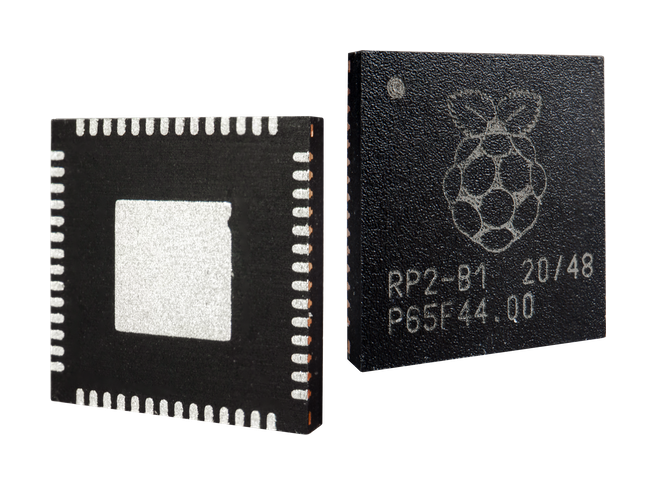
\includegraphics[width=.4\linewidth,height=.3\linewidth]{images/rp2040.png}
\end{figure}
\end{frame}

\begin{frame}{Raspberry Pi Pico}
\begin{figure}
	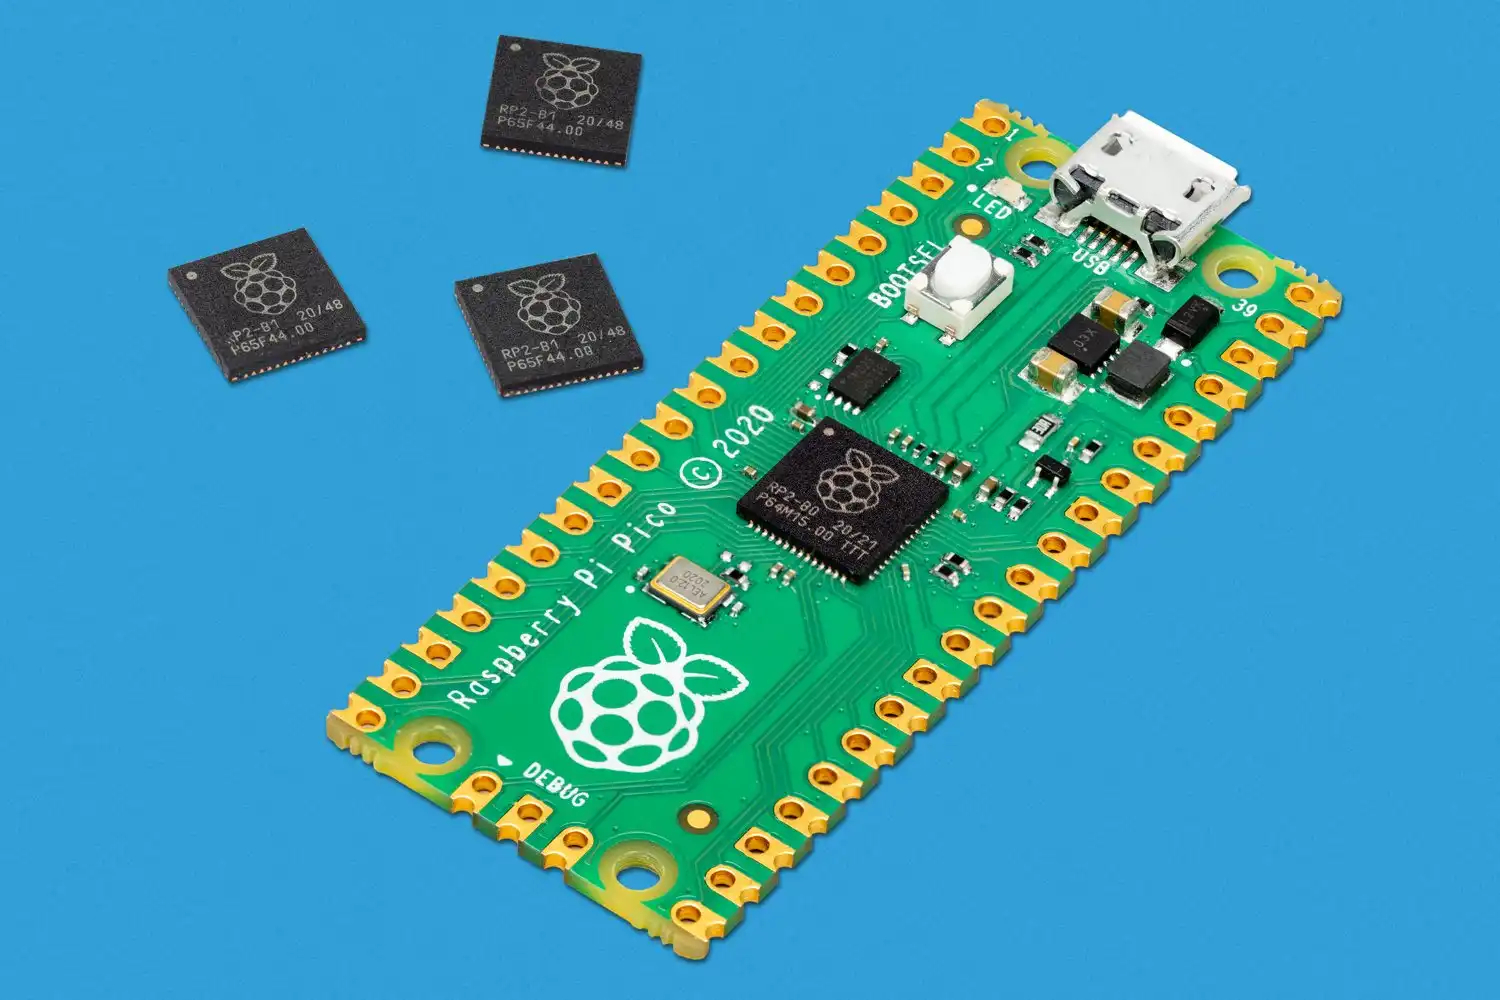
\includegraphics[width=.9\linewidth,height=.7\linewidth]{images/pico-rp2040.jpg}
\end{figure}
\end{frame}

\section{Picoprobe}
\begin{frame}{Picoprobe}
	\begin{block}{What is Picoprobe?}
		"Picoprobe allows a Pico / RP2040 to be used as USB to SWD and UART bridge. This means it can be used as a debugger and serial console for another Pico." -- Raspberry Pi LTD.
	\end{block}
\begin{figure}
	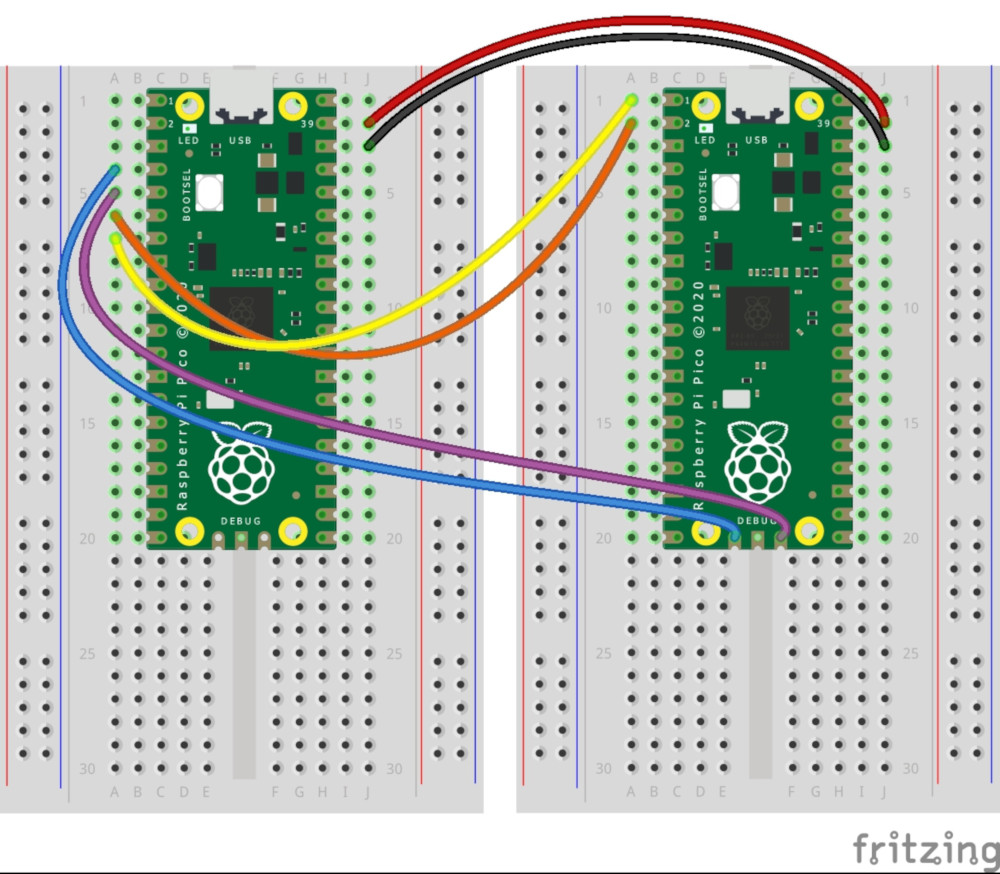
\includegraphics[width=.6\linewidth,height=.7\linewidth]{images/picoprobe_connection.jpeg}
\end{figure}
\end{frame}

%
%	\begin{frame}
%		\frametitle{Multiple Columns}
%		\begin{columns}[c] % The "c" option specifies centered vertical alignment while the "t" option is used for top vertical alignment
%			
%			\column{.45\textwidth} % Left column and width
%			\textbf{Heading}
%			\begin{enumerate}
%				\item Statement
%				\item Explanation
%				\item Example
%			\end{enumerate}
%			
%			\column{.5\textwidth} % Right column and width
%			Lorem ipsum dolor sit amet, consectetur adipiscing elit. Integer lectus nisl, ultricies in feugiat rutrum, porttitor sit amet augue. Aliquam ut tortor mauris. Sed volutpat ante purus, quis accumsan dolor.
%			
%		\end{columns}
%	\end{frame}
%	
%	%------------------------------------------------
%	
%	
%	\section{Second Section}
%	%------------------------------------------------
%	
%	\begin{frame}
%		\frametitle{Table}
%		\begin{table}
%			\begin{tabular}{l l l}
%				\toprule
%				\textbf{Treatments} & \textbf{Response 1} & \textbf{Response 2}\\
%				\midrule
%				Treatment 1 & 0.0003262 & 0.562 \\
%				Treatment 2 & 0.0015681 & 0.910 \\
%				Treatment 3 & 0.0009271 & 0.296 \\
%				\bottomrule
%			\end{tabular}
%			\caption{Table caption}
%		\end{table}
%	\end{frame}
%	
%	%------------------------------------------------
%	
%	\begin{frame}
%		\frametitle{Theorem}
%		\begin{theorem}[Mass--energy equivalence]
%			$E = mc^2$
%		\end{theorem}
%	\end{frame}
%	
%	%------------------------------------------------
%	
%	\begin{frame}[fragile] % Need to use the fragile option when verbatim is used in the slide
%		\frametitle{Verbatim}
%		\begin{example}[Theorem Slide Code]
%			\begin{verbatim}
%				\begin{frame}
%					\frametitle{Theorem}
%					\begin{theorem}[Mass--energy equivalence]
%						$E = mc^2$
%					\end{theorem}
%			\end{frame}\end{verbatim}
%		\end{example}
%	\end{frame}
%	
%	%------------------------------------------------
%	
%	\begin{frame}
%		\frametitle{Figure}
%		Uncomment the code on this slide to include your own image from the same directory as the template .TeX file.
%		%\begin{figure}
%		%\includegraphics[width=0.8\linewidth]{test}
%		%\end{figure}
%	\end{frame}
%	
%	%------------------------------------------------
%	
%	\begin{frame}[fragile] % Need to use the fragile option when verbatim is used in the slide
%		\frametitle{Citation}
%		An example of the \verb|\cite| command to cite within the presentation:\\~
%		
%		This statement requires citation \cite{p1}.
%	\end{frame}
%	
%	%------------------------------------------------
%	
%	\begin{frame}
%		\frametitle{References}
%		\footnotesize{
%			\begin{thebibliography}{99} % Beamer does not support BibTeX so references must be inserted manually as below
%				\bibitem[Smith, 2012]{p1} John Smith (2012)
%				\newblock Title of the publication
%				\newblock \emph{Journal Name} 12(3), 45 -- 678.
%			\end{thebibliography}
%		}

     % https://www.analog.com/en/analog-dialogue/articles/introduction-to-spi-interface.html
     % https://www.analog.com/en/analog-dialogue/articles/uart-a-hardware-communication-protocol.html
     % https://www.analog.com/en/technical-articles/i2c-primer-what-is-i2c-part-1.html
%	\end{frame}
%	
%	%------------------------------------------------
	
	\begin{frame}
		\Huge{\centerline{Thank you}}
	\end{frame}
	
	%----------------------------------------------------------------------------------------
	
\end{document} 